\documentclass[tikz,border=10pt]{standalone}
\begin{document}
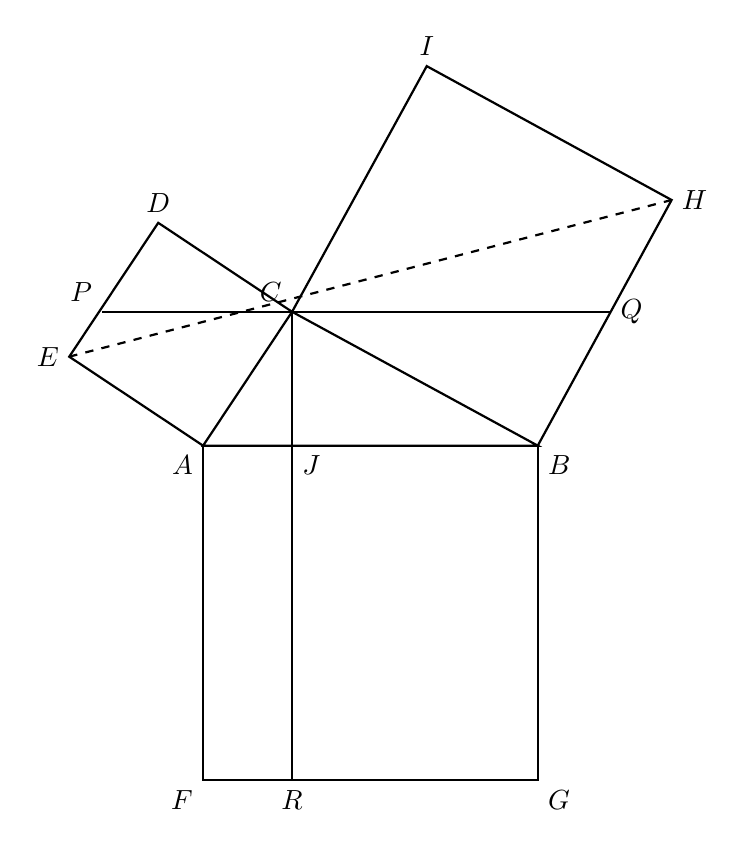
\begin{tikzpicture}[thick]
\coordinate (A) at (2.73,4.25);
\coordinate (B) at (6.98,4.25);
\coordinate (C) at (3.86,5.95);
\coordinate (D) at (2.16,7.08);
\coordinate (E) at (1.03,5.38);
\coordinate (F) at (2.73,0);
\coordinate (G) at (6.98,0);
\coordinate (H) at (8.68,7.37);
\coordinate (I) at (5.57,9.07);
\coordinate (J) at (3.86,4.25);
\coordinate (P) at (1.45,5.95);
\coordinate (Q) at (7.90,5.95);
\coordinate (R) at (3.86,0);

\draw (A) -- (B) -- (C) -- cycle;
\draw (A) -- (E) -- (D) -- (C);
\draw (C) -- (I) -- (H) -- (B);
\draw (A) -- (F) -- (G) -- (B);
\draw (C) -- (R);
\draw (P) -- (Q);
\draw[dashed] (E) -- (H);

\node[above left] at (C) {$C$};
\node[above] at (D) {$D$};
\node[left] at (E) {$E$};
\node[above left] at (P) {$P$};
\node[right] at (Q) {$Q$};
\node[right] at (H) {$H$};
\node[above] at (I) {$I$};
\node[below left] at (A) {$A$};
\node[below right] at (B) {$B$};
\node[below right] at (J) {$J$};
\node[below left] at (F) {$F$};
\node[below right] at (G) {$G$};
\node[below] at (R) {$R$};
\end{tikzpicture}
\end{document}
